\section{A different model: chronological quantization and saturation}\label{sec:maps}
\subsection{The event rule and exactness boundary}
The original finite-range operation, applied to each of the five coordinates after \emph{every event}, is
\begin{equation}\label{eq:quantizer}
 \qbox(v)=\Delta\,\clip\bigl(\rint(v/\Delta),-K,K-1\bigr),
 \qquad \Delta=\frac{2H}{2^b},\quad K=2^{b-1}.
\end{equation}
Here $\rint$ is nearest-integer rounding with ties to even, $H=2$ unless explicitly varied, and $b\in\{8,12,16\}$. Set $\lambda=-K$, $\upsilon=K-1$. The interval is asymmetric: $[-2,2-\Delta]$ in coefficient units. Its sign, range and fixed phase origin are retained.

For a quantized coordinate $\Delta k$ and unrounded event increment $v$, the ideal code update is
$k'=\clip(\rint(k+v/\Delta),\lambda,\upsilon)$.
Translation reduces this to a rounded integer addition only away from half ties. If $m-\tfrac12<v/\Delta<m+\tfrac12$, then adding integer $k$ places it strictly in the cell of $k+m$. At a tie the statement is false: $\rint(1+\tfrac12)=2$, whereas $1+\rint(\tfrac12)=1$. Floating addition can introduce an additional boundary qualification.

For the baseline constants
\begin{equation}\label{eq:cs}
 c_0=\frac{B_1}{4}\sqrt{3/7},\qquad
 s_0=\frac{B_1}{4}\sqrt{4/7},\qquad
 a=\rint(c_0/\Delta),\ b_0=\rint(s_0/\Delta),\
 p=a+b_0,\ d_0=b_0-a,
\end{equation}
the accepted rational certificates place every scaled constant strictly inside its stated rounding cell.~\cite{Mechanism} Table~\ref{tab:codes} records the consequences, with $w=\rint(B_1/(4\Delta))$.
\begin{table}[ht]\centering
\begin{tabular}{rrrrrrrrr}\toprule
$b$&$a$&$b_0$&$p$&$d_0$&$w$&$m_*$&$J$&$g$\\\midrule
8&10&12&22&2&16&12&6&253\\
12&167&193&360&26&255&12&7&101725\\
16&2673&3086&5759&413&4083&12&7&26830264\\\bottomrule
\end{tabular}
\caption{Certified baseline codes and derived bounds. $m_*$ is a sufficient same-label corner entrance count; $J$ bounds the restricted suffix family; $g=(K-1)^2-(K-d_0)^2$. These algorithmic counts have no inferred geometric meaning.}
\label{tab:codes}
\end{table}
Appendix~\ref{app:rational} states the rational enclosure construction and useful outward intervals. The source's 2,795,520 finite binary64 transition comparisons covered every incoming \emph{scalar} code for the admitted quarter-lag event types, coordinates, bases and widths. This exploits separability; it is neither a product-grid enumeration nor an all-platform transcendental proof. Our ideal-map statements use the certified mathematical codes. The large machine-grid checker is not rerun here.

\subsection{Deriving the actual pair maps}
The four harmonic event increments are obtained directly from \eqref{eq:event}:
\begin{equation}\label{eq:events}
\begin{array}{c|c|c}
\text{pair}&\text{early event}&\text{late event}\\\hline
\mathrm{LQ}&(c_0,-s_0,c_0,s_0)&(s_0,-c_0,-s_0,-c_0)\\
\mathrm{UQ}&(c_0,s_0,c_0,-s_0)&(-s_0,-c_0,s_0,-c_0).
\end{array}
\end{equation}
Each also adds $1/2$ to the mean. Completion order equals onset order for unit durations, so the late update is composed after the early update. Clipping the sum instead would change the algorithm.

\begin{theorem}[Chronological integer compositions]\label{thm:pairmaps}
On a harmonic code block $(r,i)\in[\lambda,\upsilon]^2$, define
\begin{equation}\label{eq:AB}
 \begin{aligned}
 \Amap(r,i)&=\bigl(\min(\upsilon,r+p),\ \max(\lambda,i-p)\bigr),\\
 \Bmap(r,i)&=\bigl(\max(\lambda,\min(\upsilon-b_0,r-d_0)),\
                         \min(\upsilon-a,i+d_0)\bigr).
 \end{aligned}
\end{equation}
For the certified codes, the event-wise LQ and UQ pair maps are
$\Pair_+=(\Amap,\Bmap)$ and $\Pair_-=(\Bmap,\Amap)$ on the plus/minus blocks. The mean code after a pair is $\min(\upsilon,k_\mu+2^{b-2})$.
\end{theorem}
\begin{proof}
Write $S_v(k)=\clip(k+v,\lambda,\upsilon)$. On the LQ active block the real updates are $+a,+b_0$ and the imaginary updates $-b_0,-a$. Positive increments compose as $S_{b_0}S_a(r)=\min(\upsilon,r+a+b_0)$; negative ones give the lower-saturating counterpart.

On its inactive block, real updates are $+a,-b_0$. Thus
$S_{-b_0}S_a(r)=\max(\lambda,\min(\upsilon,r+a)-b_0)
=\max(\lambda,\min(\upsilon-b_0,r-d_0))$.
Imaginary updates are $+b_0,-a$. Their composition is
$\max(\lambda,\min(\upsilon-a,i+d_0))$; the lower maximum is redundant since $i+d_0\ge\lambda$ and $\upsilon-a\ge\lambda$. This yields $\Bmap$. The UQ table exchanges active and inactive blocks. Each mean increment is exactly $(1/2)/\Delta=2^{b-3}$ code units; two positive increments give the displayed cap.
\end{proof}
The upper truncation $\upsilon-b_0$ in $\Bmap$ is an intermediate-event effect, not an arbitrary bound. At incoming real code $\upsilon$,
\[
 S_{-b_0}S_a(\upsilon)=\upsilon-b_0,\qquad
 S_aS_{-b_0}(\upsilon)=\upsilon-b_0+a .
\]
They differ. Repeated saturation destroys commutation and can retain an order-sensitive distinction that an additive sum loses.

\subsection{A sufficient corner mechanism}
Let $C_*=(\upsilon,\lambda)$ and $V=\norm{C_*}^2=(K-1)^2+K^2$.

\begin{theorem}[Incoming-state corner dominance]\label{thm:corner}
For any one of the three baseline widths, suppose the active incoming block of the final pair satisfies
\begin{equation}\label{eq:entry}
 r\ge\upsilon-p,\qquad i\le\lambda+p,
\end{equation}
and the other block is anywhere in the code square. Then the final active block is $C_*$ and the fixed directional readout has the correct sign. More precisely,
\begin{equation}\label{eq:margin}
 \ell\etaosc\ge\frac{g}{2V-g}>0,\qquad
 g=(K-1)^2-(K-d_0)^2 .
\end{equation}
\end{theorem}
\begin{proof}
The formula for $\Amap$ proves $C_*$ under \eqref{eq:entry}. Every $\Bmap$ output belongs to
$[\lambda,\upsilon-b_0]\times[\lambda+d_0,\upsilon-a]$.
For the listed constants $0<b_0<K$, so the real absolute value is at most $K$. Also $d_0>1$ and $d_0\le a+1$, so both imaginary endpoints have absolute value at most $K-d_0$. Thus $\norm{\Bmap}^2\le K^2+(K-d_0)^2=V-g$, and $g>0$. The label-signed ratio is $(V-q)/(V+q)$ for $q=\norm{\Bmap}^2\ge0$. This function decreases with $q$, giving \eqref{eq:margin}. All listed lower bounds lie well above the fixed arithmetic band.
\end{proof}
Every retained directional endpoint in the 48-history subset satisfies this sufficient active-corner condition at all three widths. That is a mechanism for the observed subset, not an assertion that every incoming history meets \eqref{eq:entry}.

\begin{proposition}[Twelve consecutive pairs and a restricted suffix regime]\label{prop:suffix}
From any harmonic code square, $m_*=\lceil(2K-1)/p\rceil=12$ consecutive identical baseline labels suffice to put their active block at $C_*$. Define
\begin{equation}\label{eq:Dk}
 D_k=\Bmap^k(C_*)=
 \left(\max(\lambda,\upsilon-b_0-(k-1)d_0),\
             \min(\upsilon-a,\lambda+kd_0)\right)\quad(k\ge1).
\end{equation}
For $1\le k\le J=1+\lfloor a/d_0\rfloor$ one has $\Amap(D_k)=C_*$. Here $J=6,7,7$. Consequently, states $(C_*,D_k)$ and $(D_k,C_*)$ have a conditional suffix description: repeating the current label increments $k$, while reversing the label resets to the exchanged state with $D_1$, provided every such use stays in $k\le J$.
\end{proposition}
\begin{proof}
Iteration gives $\Amap^m(r,i)=(\min(\upsilon,r+mp),\max(\lambda,i-mp))$. The maximum required coordinate travel across the square is $2K-1$, proving the sufficient count. For \eqref{eq:Dk}, the first inactive real step is $\upsilon-b_0$, then each step decreases by $d_0$ until the lower cap. The imaginary coordinate rises by $d_0$ until its upper cap. Induction proves the formula. The real entry requirement for $\Amap(D_k)$ is
$\upsilon-b_0-(k-1)d_0\ge\upsilon-p$, equivalently $(k-1)d_0\le a$.
The imaginary requirement follows from $kd_0\le a+d_0=b_0\le p$. For these widths the relevant values do not hit a cap that invalidates either inequality. Thus $\Amap(D_k)=C_*$. Now $\Amap(C_*)=C_*$ and $\Bmap(C_*)=D_1$; substitution into the two pair maps proves both conditional transitions.
\end{proof}
This does not assert entrance into the short-suffix family from every history. A long run can push its inactive block beyond the stated $J$ regime even though its active block remains at the corner. Twelve is a sufficient corner-entry count, not a minimal decision time, one-write replacement theorem or a count of physical openings.

\begin{figure}[ht]
\centering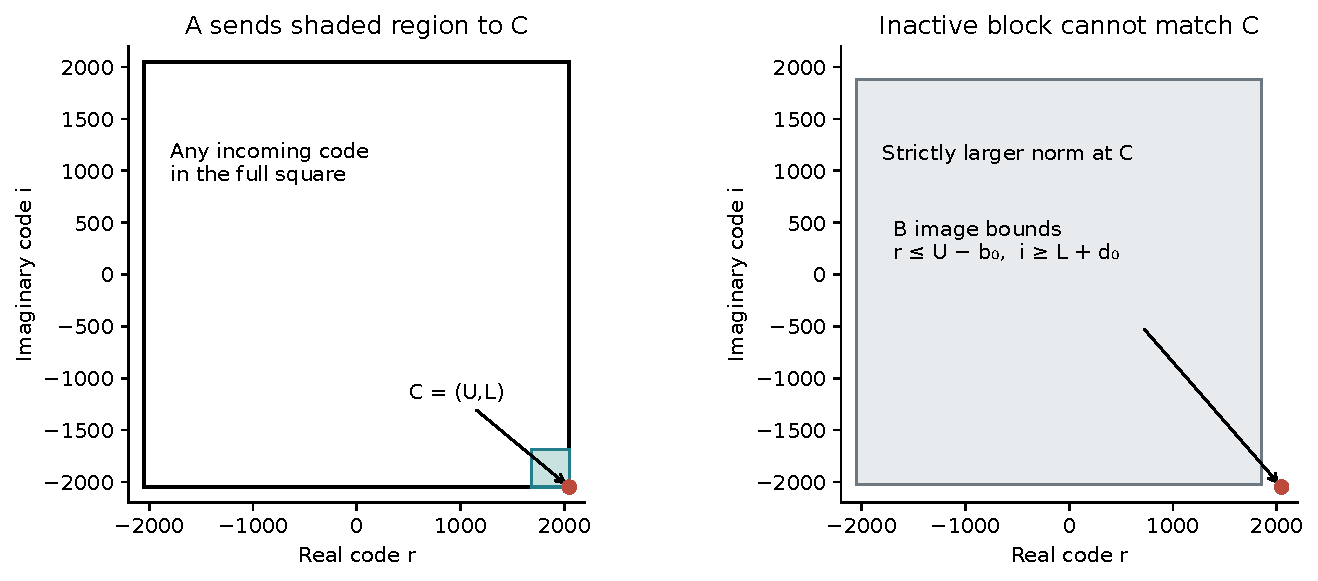
\includegraphics[width=\linewidth]{figures/fig04_corner.pdf}
\caption{Numerical code geometry at 12 bits; diagram labels $U=\upsilon$, $L=\lambda$, $C=C_*$. The final active map collapses its shaded incoming region to $C_*$. The inactive image has strictly smaller maximum norm. These rectangles depict numerical state space, not the toroidal construction.}
\label{fig:corner}
\end{figure}

\subsection{Independent Fourier clipping and same-operator conjugacy}
\begin{theorem}[Fourier corner abstention]\label{thm:fouriercorner}
For zero-start aligned quarter pairs under independent event-wise Fourier-axis quantization, let $n_+,n_-$ be the order counts. In code units,
\begin{equation}\label{eq:fouriercorner}
 \begin{aligned}
 z_U/\Delta&=-\min(K,n_+w)+\ii\min(\upsilon,n_-w),\\
 z_L/\Delta&=-\min(K,n_-w)+\ii\min(\upsilon,n_+w).
 \end{aligned}
\end{equation}
If both counts are at least $q_*=\max(\lceil K/w\rceil,\lceil\upsilon/w\rceil)$, equal to $8,9,9$ at the three widths, both moments equal $-K+\ii\upsilon$ in code units and the readout abstains.
\end{theorem}
\begin{proof}
An early aligned event adds the negative real moment $-B_1/4$, and a quarter-late event adds the positive imaginary moment $\ii B_1/4$. Port U is early on LQ and late on UQ, with the opposite assignments at L. Each affected coordinate therefore moves only one way, so repeated saturation is the capped count in \eqref{eq:fouriercorner}. The thresholds make both ports identical. Their cross product is real, so the numerator in \eqref{eq:momentread} is zero; the denominator remains positive by invertibility.
\end{proof}
All retained length-128 fixed-point histories meet both thresholds. Their complete state is $(\upsilon\Delta,(-K+\ii\upsilon)\Delta,(-K+\ii\upsilon)\Delta)$. Zero correct means 48 abstentions, not 48 reversed answers.

\begin{theorem}[Transporting the operator]\label{thm:conjugacy}
Let $Q$ be any fixed operation on the directional real state and $x=\Tp y$. If increments satisfy $v=\Tp w$, then the moment-coordinate operation
\begin{equation}\label{eq:conjugacy}
 y'=\Tp^{-1}Q\bigl(\Tp(y+w)\bigr)
\end{equation}
gives exactly $\Tp y'=Q(x+v)$. Applying the same axis-aligned coordinate quantizer independently to $y$ instead is generally a different nonlinear map.
\end{theorem}
\begin{proof}
Substitute $x=\Tp y$ and $v=\Tp w$, then multiply by $\Tp$. Since $\Tp$ is invertible, adjacent inverse factors cancel, proving equality at each event and by induction along every finite event list. Independent coordinate clipping would require $Q\Tp=\Tp Q$, which is false for a general mixing matrix: the inverse image of an axis box is an oblique cell set, not that same box.
\end{proof}
The saved conjugated control agrees after mapping back within $6.67\,10^{-16}$ at all 384 checkpoints, with identical decisions. Its transformed floating coordinates are not five independent $b$-bit Fourier values.

A common onset shift $\phi$ actively rotates both harmonic amplitudes by $e^{-2\pi\ii\phi}$. Lossless norms are invariant. A fixed asymmetric axis box is not generally rotation-covariant: even reversal of a boundary value can fall at the missing positive endpoint. A passive coordinate change $x'=Rx$ must transport increments, readout and box as $Q'=RQR^{-1}$. The frozen common-phase controls rotate the inputs relative to a fixed box; they are active tests, not passive relabellings or trial-specific rephasing.
